\documentclass[twoside,a4paper,12pt,english]{inac17}

%INAC2017 SETUP: SET PAGE SIZE AND SET FOR USING graphicx PACKAGE.
\usepackage{graphicx}
\usepackage{babel,varioref,epsfig} %,rotating}
\usepackage{amssymb}
\usepackage[font=bf,center]{caption}
\usepackage{subfigure}

\usepackage{textcomp}             % Para usar marca registrada

\title{PROFESSIONAL CLUSTER MANAGEMENT BY A SMALL SCIENTIFIC TEAM: CHALLENGES, SOLUTIONS
AND PERSPECTIVES}

%INAC2017 SETUP: SPECIFY AUTHOR NAMES, AFFILIATION, ADDRESS AND E-MAIL.

\author{
  \bf{Vitor V. A. Silva, Andr\'e A. C. dos Santos and Renan O. Cunha}\\ \\
  CDTN - Centro de Desenvolvimento da Tecnologia Nuclear\\
  Av. Ant\^onio Carlos 6627 - Campus UFMG\\
  31270-901 - Belo Horizonte, MG\\
  \{vitors, aacs, roc\}@cdtn.br}

\begin{document}

%INAC2017 SETUP: PRINT TITLE
\maketitle

%INAC2017 SETUP: SETUP HEADS FOR PAGES
\pagestyle{myheadings}
\thispagestyle{empty}
\markboth{}{}


%INAC2017 SETUP: SET FIRST PAGE WITH NO PAGE NUMBER
\thispagestyle{empty}

%--------------------------------------------------------------------------------------

\begin{abstract_full_paper}
  The specification, configuration and management of a professional computer cluster are specialized
tasks usually hold by well trained teams, often full-time hired computer scientists. However, in
many situations and for widely different reasons, these very specific technical tasks must
be carried on by no other than the user itself. This is the situation at Centro de Desenvolvimento
da Tecnologia Nuclear - and in many nuclear research and educational centres in developing countries -
where the scientists are the users of the cluster but also the technical
team responsible to keep the system running. This paper presents the process of planning
and installing the whole operating system and scientific software of a professional cluster
aimed to be used in the nuclear engineering field from the point of view of its users.
The drawbacks of lack of expertise and technical skills to
manage such type of technology are opposed to the advantages of freedom to chose the solutions
which best fit to the problems to be solved. The details of selected methods or technologies
chosen for addressing a specific matter are presented together with other possible options, 
offering a broader view of the whole process of cluster's configuration. Specificities
of dealing with closed, restricted and open software, common in the nuclear engineering field,
are also put in perspective. The ideas and solutions presented in this paper can be a
valuable reference to other research teams found in a similar situation:
being scientists and its own technical staff at the same time.
\end{abstract_full_paper}

%--------------------------------------------------------------------------------------

\section{INTRODUCTION}\label{int}

Now days computers are indispensable tools for scientists of any field.
Some areas of research heavily rely on computational power in order to solve
complex problems by use of demanding algorithms, methods and heuristics.
Current methods used for nuclear reactor calculations, both thermal-hydraulics
and neutronics can be more accurate or even only applicable by using
many cores or computers altogether.

A computer cluster consists of set of computers connected to work together. The difference of the
definition between a computer cluster and a computer grid is that usually grids are more
heterogeneous and used to a different set of problems at the same time, while a computer
cluster is aimed to have each node solving the same problem.

To be able to have sets of computers working together and be able to control the utilization of the system,
it is absolutely fundamental to have an operating system capable of offering interconnection, data sharing,
task schedule and user administration. The \textbf{de facto} operating system widely used in these situations
is Linux \cite{linux}. After choosing a suitable operating system, its mandatory to evaluate the applications to
be used, the level of security to be enforced and, fundamentally, the dynamics of the operation of the system.
These factors will define the suitable solutions for different aspects of the system, ranging from data
sharing among nodes to options to update, backup and access the system.


%--------------------------------------------------------------------------------------

\subsection{Context}

As aforementioned, the cluster presented in this paper is aimed to scientific computing.
Since the expression scientific computing has many meanings, depending on the context, a
clarification is necessary. This cluster will be utilized to run computational fluid dynamics
(CFD) simulations, neutronics simulations - both using deterministic and Monte Carlo methods
and coupled calculations, involving the two disciplines. It is also natural to predict
its expansion in utilization to other fields depending on its demand, performance and availability.

The users of the system are mainly nuclear and mechanic engineers, scientists and graduate
and undergraduate students. These users have different levels of knowledge of the work
they must carry and also are unevenly skilled as system users. These differences must be taken
in account when planning and choosing the operational characteristics of the system.

From the perspective of the Centro de Desenvolvimento da Tecnologia Nuclear (CDTN), such system
is a fundamental asset. Computer power is, at the very end, power of calculation and any research
team with demand for intensive computing is a potential user and potential client of the cluster.
With this in mind, there is a real potential of increase of research of CDTN related to
scientific computing. An interesting perspective of the way of research can change with the
use of intensive scientific computing - in this case, the extreme computing - is elegantly
presented by Dongarra \cite{Dongarra2017}.

%Teste de todas as citações disponíveis no bibtex: Wu\cite{Wu2016}, Nagaya\cite{Nagaya2015}.

%------------------------------------------------------------------------------

\section{OBJECTIVE}

The objective of this paper is to present the challenges, problems and solutions proposed
to setup a professional computational cluster to carry heavy numerical calculations focused in
neutronics and thermal-hydraulics of nuclear reactors in a
context of a small research team.

%\begin{equation}
%  \nabla\cdot\mathbf{J} + \Sigma_{a} \Phi - s =0 .
%  \label{eq_1}
%\end{equation}

%------------------------------------------------------------------------------

\section{METHODS AND PROCEDURES}

\subsection{Local Structure}

In order to start the operation of a cluster system, there are some considerations the must
be taken in account. The physical location of the system is fundamental for safe, secure and
reliable operation.

From the security point of view, the cluster is located at a locked room with limited access to
the personal related to manage and install the system. The building in which the cluster is located
is part of the entire institute which is fenced and guarded by armed security personal, what makes
unautorized access or intrusion a minor issue.

The meaning of safety in this text is related to only to system safety. Personal
safety is not an issue since no special conditions are necessary to operated and use the cluster other
than use an ordinary desktop computer. The safety of the system consist in guarantee environmental conditions
which are not harmful to the hardware. In order to guarantee a proper operational temperature, two dedicated
air conditioning devices work in parallel. These equipments are dimensioned to be able to maintain, each one alone,
the working temperature at the cluster room considering the system at full operation, i.e. all nodes using all cores
and GPU's.

Related to reliability, the system is plugged to a remotely configurable no-break of 40KvA. This equipment
can provide power for the whole cluster for more than 10 minutes, time sufficent to be able to save the state of current jobs
for all users. The implementation of shutdown scripts related to no-break signais is still to be defined.

\subsection{Hardware and Software}

The so-called cluster system is formed by a set of identical high performance computers -
total number of eight machines - plus a master unit with slightly different configuration.
Figure~\ref{fig:cluster} presents a schematic representation of the system.

\begin{figure}[h] % t forces top and b forces bottom: can be added to h, ex. [ht]
  \centering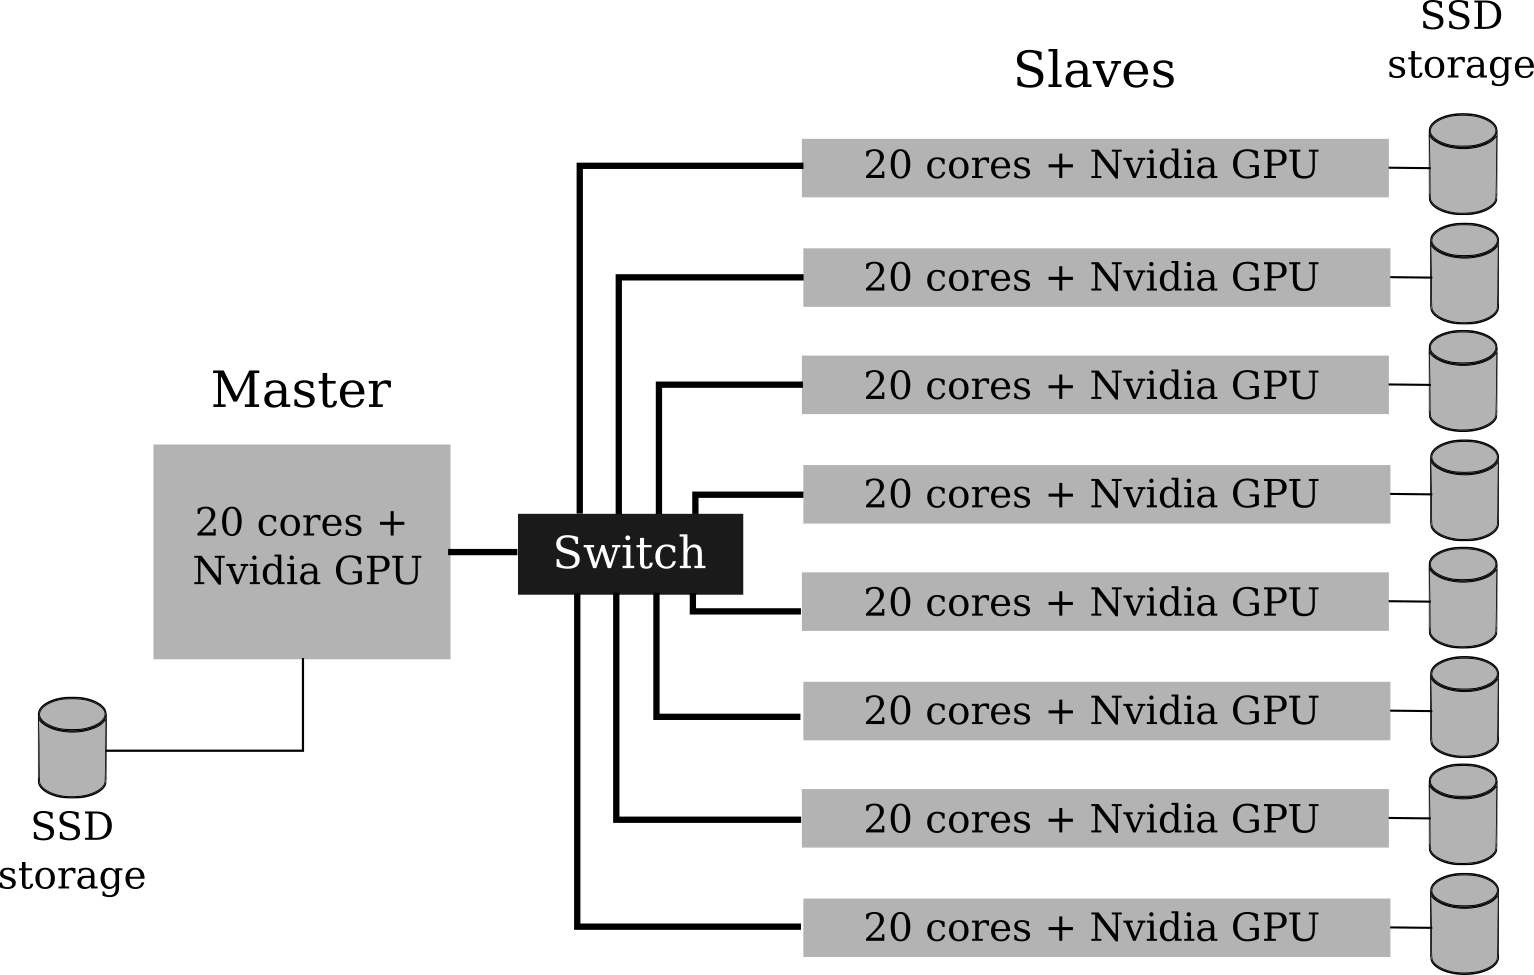
\includegraphics[scale=0.7]{images/cluster-topologico.png}
  \caption{Cluster hardware.}
  \label{fig:cluster}
\end{figure}

The \textit{slave} machines are Dell workstations Precision R7910. These machines are equipped
with Dual Intel{\textregistered} Xeon{\textregistered} processors E5-2640 operating at $2.4$GHz with
$32$Gb of RAM each. They have 2x$10$GbE (Gigabit Ethernet) and 2x$1$Gbit network connectors, which
allow the use of the Gigabit network exclusively for intra-cluster communication. Each node
has a $360$Gb solid state disk for storage.

These equipments are also installed with Nvidia{\textregistered} GPU's (Graphic Processing Units) M4000{\textregistered} with $8$Gb CUDA\cite{CUDA} capable.
The GPU's on nodes, despite capable of visualization, are expected to be used as secondary calculation units.
The use of graphic processors for calculations is widely applied in scientific computing and these divides
are also called accelerators \cite{accelerators}.

The \textit{master} machine is a Dell Precision T7910, with very similar configuration of the slaves. The main
differences rely on the graphics processor unit, equipped with another Nvidia{\textregistered} GPU: a
Quadro{\textregistered} M2000 with $4$Gb of memory. These video card is not aimed for calculations, but for
visualization of data and graphics display. The other different is in the main RAM memory, having the \textit{master}
$256$Gb of RAM. 

A set of three hard-disks of $500$Gb was installed to the master node, making an extra $1.5$Tb to be used as part
of the distributed file system.

The original OS sold with the cluster is an OEM (Original Equipment Manufacturer) Windows 7{\textregistered} \cite{windows7}. This
OS is not supported by the whole set of software expected to be used by the research group users. The chosen
system to replace the original Windows 7 is CentOS (Community Enterprise Operating System)\cite{centos}, which offers a platform to natively run all
software needed by the users. Details on possible options for software compatibility and operating system independence will be given on subsection \ref{sub:ssol}

\subsection{Linux Operating System}

The reason for choosing \textit{CentOS} as the Linux flavor for the system is due to its characteristics and the previous
experience of the cluster management team. CentOS is aimed to offer a free, enterprise-class, community-supported computing
functionality. It appeared as a fork of Red Hat Enterprise Linux, which is available only trough paid subscription. The option
for CentOS, in this context, is to have both the strong development for enterprise systems and also its gratuity.

A second reason is to take advantage of previous competence of the installation and user team which already has experience
in using Fedora Linux, a distribution fully compatible with CentOS.

That said, all the software currently in use by the Thermal-Hydraulics Laboratory team are compatible with CentOS. This
makes this flavor of Linux the straighforward choice for the cluster system. It is also worth noting that the use of
free and open-source software has a social meaning in promoting the share of knowledge.

\subsection{Software Solutions}
\label{sub:ssol}

Before choosing a software for perform a desirable task, its mandatory to have a consistent definition of the environment
in which the system will be used. The first constraint is the network environment. It's worth noting that the cluster is
located in the CDTN network and the restrictions and security rules enforced in the network must be followed by the system.

With this is mind, the choice is to have the system - the slave machines - in one isolated sub-network only accessed by
the master node. The master node is part of both the sub-network and the institute's network. The sole point of access to the
internet for any slave is the master node which, in turn, is connected to the internet using a proxy connection and a
NAT (Network Access Translation). The topology of the cluster network is presented in Figure ~\ref{fig:esquema-cluster}.

\begin{figure}[h] % t forces top and b forces bottom: can be added to h, ex. [ht]
%  \centering\includegraphics[width=8.5cm,height=8.5cm]{images/esquema_cluster_edited_bw.png}
  \centering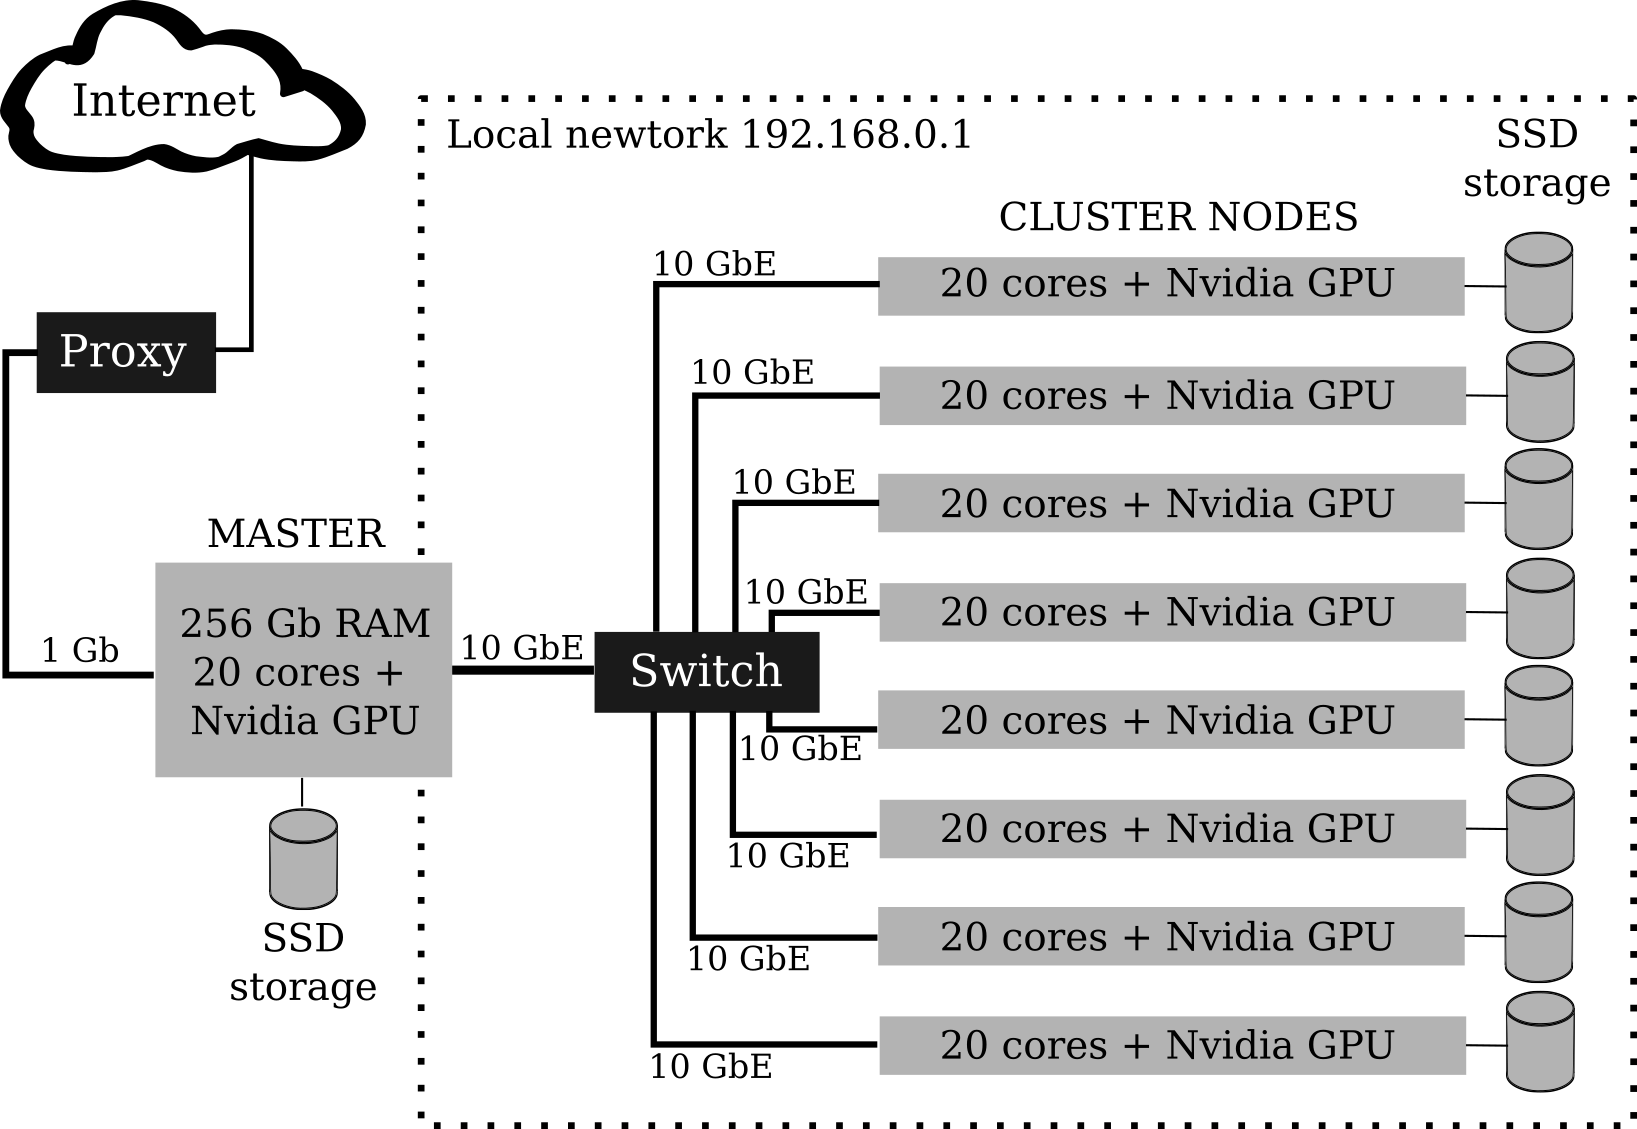
\includegraphics[scale=0.7]{images/cluster-rede.png}
  \caption{Cluster showing its network topology.}
  \label{fig:esquema-cluster}
\end{figure}

The chosen network topology have impacts on system maintenance. Since the slave machines cannot access the internet, the
master is configured to hold a mirror of packages installed in all system machines. The average download rate for the master node is of $500$Kbytes/second in
CDTN's network. The master is scheduled to make updates from time to time (once a week in the current configuration) while the slaves are also scheduled to
make their updates after the master and from it. This approach has advantages, like decreasing internet bandwitch demand since only
one machine downloads updated packages from the internet. Other advantage is in downloading time, since the slaves
use dedicated $10$GbE connections to the master which provides the necessary packages. The drawback is the amount of disk space needed to keep a mirror of CentOS packages locally.
To decrease the space consumption, only packages already installed on the system - master and slaves - are
downloaded. In the case of the installation of a new package, it must be installed in the master. After that,
the scheduled script guarantees its availability for the slaves.

\subsection{File System}

A crucial element of a computer system architecture is its file system. A file system is the set of data structures and functions an operating system
use to manage and keep track of files on disks and partitions. There is a large number of file systems being used by different operating systems\cite{linuxbook}.

However, in a high performance and high demand system like a cluster, there are some desirable features not usually provided for standard computers file systems.
For example, the ability to have many different interconnected computers reading and writing information concurrently and asynchronously. These kind of feature
is provided by a specialized file system, usually called distributed file system\cite{hal}.

The chosen solution for distributed file system management is the GlusterFS\cite{gluster}. GlusterFS is an open source, distributed file system and has
a unique no-metadata server architecture. Most distributed file systems use a metadata server, which has information on where to retrieve data which is
physically scattered among different disks. This architecture imposes a dependence on the metadata server. If it goes down, the system becomes inacessible.
GlusterFS keeps this information as distributed hashes, avoiding the dependence on one server or node.

The control of Gluster is transparent for users, providing a level of abstraction with no impact on how users of the system operate with their files. This
abstraction also has no impact in system management. An envisaged quota control of user accounts can work without any problem above the GlusterFS file system.

Another option under consideration is the more robust Lustre file system\cite{lustre}. Lustre is a parallel distributed file system widely used in large-scale
cluster systems. Despite its reliability and recognized performance (high I/O troughput: more than a terabyte per second), it is not the first choice due to its higher operating dificulties compared to GlusterFS.
The size of the presented cluster is also small by Lustre standards. However, it remains as a second option in the case of GlusterFS does not perform as expected. 

However, there are more than one way of setup a cluster system with respect
to file system, software execution and user access.

The next sub-sections describe alternatives to the use of a direct Linux operating system. They are not current used but remain as options
in the case of, for example, software incompatibility. 

\subsubsection{Dockers}


\subsubsection{Operating System Virtualization}

\subsection{Visualization}

The presence of powerful GPU devices in each node of the cluster make possible their use for calculations. However,
this hardware can be used for its natural task: visualization. At a first glance, this can sound natural and
straightforward. However, there are trick details in using different nodes to render and output one image. The first one
is the ability to gather scattered information in order to produce the desirable output in one display.

Gladly, there is software aimed to data visualization which address the presented issue. Developed by Kitware\cite{kitware},
Paraview\cite{paraview} is an open-source multiple-platform application for scientific visualization. Its design considers
the use of a client-server architecture in order to deal with data-sets scattered among many nodes in a multiprocessing
system. 


\subsection{Graphics Processors: Extended Use}
%\subsection{Extending the Use of graphics processors}

The system under consideration has powerful GPU cards installed in machines
which have no output display. The use of GPU's to perform tasks other than graphics processing
is nowadays widespread in many fields of research \cite{UsoDeGpus}. Modern software is written with
the objective of taking advantage of this ``extra'' processing capabilities and studies of software
engineering on parallelization of sequential algorithms to be applied in GPU's are a significant
nowadays.

In order to make the use of GPU's for general processing less difficult, libraries, compilers and
frameworks were developed. At the beginning these tools were developed and deployed by graphics cards
manufacturers. The pioneer in offering both GPU's cards capable of general use is NVIDIA, which,
without surprise, is also pioneer in making a available a full framework for its GPU programming.
This tool is called CUDA (Compute Unified Device Architecture) and is a ``de facto'' parallel computing platform
and application programming interface (API) model.

CUDA can be used with a set of libraries for ...........

However, with the increase of the use the cards, developers start to demand some
standardization in order to be able experiment new algorithms in different cards. Today, the
reference framework for development for heterogeneous platforms is \textit{OpenCL} \cite{OpenCL}.

--- Como funciona o OpenCL

The idea for the cluster system, is to provide both CUDA libraries for
software developed for NVIDIA graphic cards and also OpenCL libraries to
be used by software written to make use of the programming genericity
provided by OpenCL. As the time of writing, the libraries were installed
in only one node of the cluster and tests are being envisaged to check
compatibility of both frameworks.





\section{RESULTS AND ANALYSIS}

The current status of the system is that is it not yet operational.
\begin{itemize}

\item (Situação atual do sistema - no momento de finalizer o paper)
\item (Dificuldades identificadas: Resolvidas (como) e Pendentes.
  
\end{itemize}

%------------------------------------------------------------------------------
\subsubsection{Sub-subsection level and lower: only first character uppercase}

Figures and tables should appear as closely as possible to where they are first cited, e.g. Fig.~\ref{fig:esquema-cluster}, in the text.  Figures are numbered in Arabic numerals, with the caption centered below the figure, in boldface. Double-space before the figure, and after the figure caption.


\newcommand{\cc}{\centering}
\newcommand{\rr}{\raggedright}
\newcommand{\tn}{\tabularnewline}
\renewcommand{\arraystretch}{1.5}
\begin{table}[h]
\caption{Numerical results to the model problem} %title of the table
\centering % centering table
\begin{tabular}{|p{3cm}|p{2cm}|p{2cm}|p{2cm}|p{2cm}|}
\hline
\cc Mesh             &\cc 8$\times$8  &\cc 16$\times$16   &\cc 32$\times$32   &\cc 64$\times$64 \tn \hline        
\rr Nodal            &\cc 1.000       &\cc 2.500          &\cc 6.250          &\cc 1.563        \tn \hline
\rr Characteristic   &\cc 1.000       &\cc 2.500          &\cc 6.250          &\cc 1.563        \tn \hline
\end{tabular}
\label{table_1}
\end{table}

When importing figures or any graphical image please verify two things:

\begin{itemize}

\item Any number, text or symbol is in Times font and is not smaller than 10-point after reduction to the actual window in your paper;

\item That it can be translated into PDF.

\end{itemize}



Tables, like Table~\ref{table_1}, are numbered in Arabic numerals, with the caption centered above the table, in {\bf boldface}.  Double-space before and after the table.

%------------------------------------------------------------------------------

\section{CONCLUSIONS AND PERSPECTIVES}

(O que está bom, o que está ruim na atual instalação)
(Trabalhos futuros: pra onde ir (operação), possíveis mudanças)

There are many ongoing tasks and even more tasks still to be started. To mention a few, one
interesting task related to the reliability and data management is the implementation of
a automatic process of shutdown on loss of power supply.

%Uma cita\c{c}\~{a}o \cite{Henderson17}.


%------------------------------------------------------------------------------



\section*{Acknowledgments}
The authors would like to thank FUJB for financing the cluster acquisition
as part of the project \textit{Desenvolvimento de novos elementos combust\'{i}veis nucleares
  e materiais e pe\c{c}as para combust\'{i}veis nucleares}, agreement FINEP 01.07.0548.00 - Process FUJB 13.867-3.
The authors also thank Dr. Jo\~{a}o Roberto Loureiro de Mattos for the work which made possible the acquisition
of the cluster.

%%%%%%%%%%%%%%%%%%%%%%%%%%%%%%%%%%%%%%%%%%%%%%%%%%%%%%%%%%%%%%%%%%%%%%%%%%%%%%%%%%%%%%%%%%%%

\begin{thebibliography}{99} %99 é o número máximo que o thebibliography permite. Numero de referencias que aparecerão.

\bibitem{linux} ``The Linux Documentation Project'', \\\verb#http://www.tldp.org/LDP/intro-linux/html/chap_01.html# (2017).

\bibitem{Dongarra2017} John Dongarra et. al., ``With Extreme Computing, the Rules Have Changed'', \textit{Computing in Science Engineering}, \textbf{19}, pp. 52--62, (2017).

\bibitem{accelerators} ``What is GPU-accelerated computing?'', \\\verb#http://www.nvidia.com/object/what-is-gpu-computing.html# (2017).

\bibitem{windows7} Jorge Orchilles, \textit{Microsoft Windows 7 Administrator's Reference}, Syngress, Boston USA (2010).

  % author = {Wirzenius, Lars},
% title = {The  Linux System Administrator's Guide},
% year = {2000},
% isbn = {0595137636},
% publisher = {iUniverse, Incorporated},
%} 

  % Centos
  
\bibitem{linuxbook} Wirzenius and Lars, \textit{The  Linux System Administrator's Guide}, iUniverse incorporated (2000).

\bibitem{hal} Benjamin Depardon, Ga\"{e}l Le Mahec and Cyril S\'{e}guin, ``Analysis of Six Distributed File Systems'', Research Report, pp. 44, (2013).
  
\bibitem{gluster} Alex Davies and Alessandro Orsaria, ``Scale out with GlusterFS'', \textit{The Linux Journal}, \textbf{2013}, (2013).

  % journal = {Linux J.},
% issue_date = {November 2013},
% volume = {2013},
% number = {235},
% month = nov,
% year = {2013},
% issn = {1075-3583},
% articleno = {1},
% url = {http://dl.acm.org/citation.cfm?id=2555789.2555790},
% acmid = {2555790},
% publisher = {Belltown Media},
% address = {Houston, TX},
%} 


\bibitem{CUDA} John Nickolls, Ian Buck, Michael Garland and Kevin Skadron, ``Scalable Parallel Programming with CUDA'', \textit{Queue - GPU Computing}, \textbf{6}, pp. 40--53, (2008).



  
%\bibitem{article} B. Author(s), ``Title", \textit{Journal Name in Italic}, \textbf{Volume in Bold}, pp. 34--89, (19xx).

%\bibitem{proceeding} C. D. Author(s), ``Article Title", \textit{Proceeding of Meeting in Italic}, Location, Dates of Meeting, Vol. n, pp. 134--156, (19xx).

%\bibitem{book} E. F. Author. \textit{Book Title in Italic}, Publisher, City \& Country (19xx).

%\bibitem{website} ``Spallation Neutron Source: The next-generation neutron-scattering facility for the United States", \verb#http://www.sns.gov/documentation/sns_brochure.pdf# (2002).

\end{thebibliography}

% ---------------------------------------------------------
% Minha bibliografia usando arquivo externo

%\bibliographystyle{unsrt}
%\bibliography{bibli}


\end{document}
